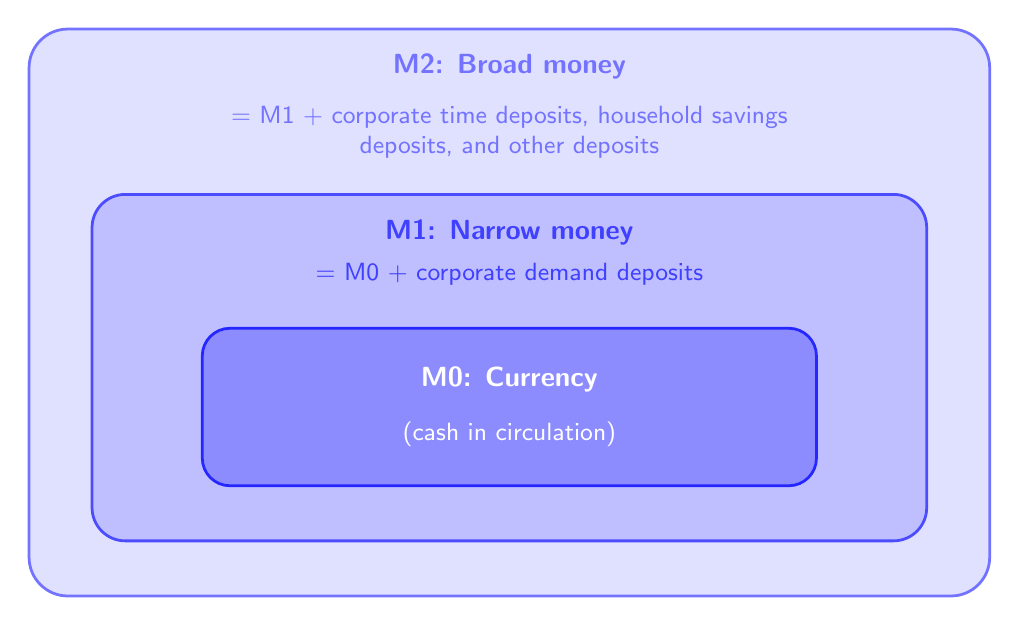
\begin{tikzpicture}[font=\sffamily]
  % Monetary aggregates as TRUE nested containment: M2 contains M1 contains M0.
  % Graduated blue shades convey the subset relation M2 \supset M1 \supset M0:
  % outermost lightest (M2), middle (M1), innermost darkest (M0).

  % --- M2: outer, lightest box (broad money) ---
  \draw[fill=blue!12, draw=blue!55, line width=1pt, rounded corners=14pt]
    (0,0) rectangle (12.2,7.2);
  \node[anchor=north, font=\sffamily\bfseries, text=blue!55] at (6.1,7.0)
    {M2: Broad money};
  \node[anchor=north, align=center, text width=11.6cm, font=\sffamily\small,
        text=blue!55] at (6.1,6.35)
    {$=$ M1 $+$ corporate time deposits, household savings\\
     deposits, and other deposits};

  % --- M1: middle box, lighter shade (narrow money) ---
  \draw[fill=blue!25, draw=blue!70, line width=1pt, rounded corners=12pt]
    (0.8,0.7) rectangle (11.4,5.1);
  \node[anchor=north, font=\sffamily\bfseries, text=blue!75] at (6.1,4.9)
    {M1: Narrow money};
  \node[anchor=north, align=center, text width=9.8cm, font=\sffamily\small,
        text=blue!75] at (6.1,4.35)
    {$=$ M0 $+$ corporate demand deposits};

  % --- M0: inner box, darkest shade (currency) ---
  \draw[fill=blue!45, draw=blue!85, line width=1pt, rounded corners=10pt]
    (2.2,1.4) rectangle (10.0,3.4);
  \node[font=\sffamily\bfseries, text=white] at (6.1,2.75)
    {M0: Currency};
  \node[align=center, text width=7.0cm, font=\sffamily\small, text=white]
    at (6.1,2.05)
    {(cash in circulation)};
\end{tikzpicture}
